\documentclass[10pt,tumble]{leaflet}
\usepackage[T1]{fontenc}
\usepackage{libertine}
\renewcommand{\familydefault}{\sfdefault}
\usepackage{microtype}
\usepackage{graphicx}
\usepackage{float}
\pagenumbering{gobble}

\title{Team 2767}
\author{\Large\textbf{Stryke Force}}

\begin{document}
\begin{center}
 \LARGE\textbf{Team 2767\\ Stryke Force}\\
 \Large{Est. 2009\\ Kalamazoo, MI}\\
 \vspace{0.5in}
 
\includegraphics[scale=0.2]{assets/strykeforce}\\
 \vspace{0.5in}
 \LARGE\textbf{Software Development Team}
 \vfill
 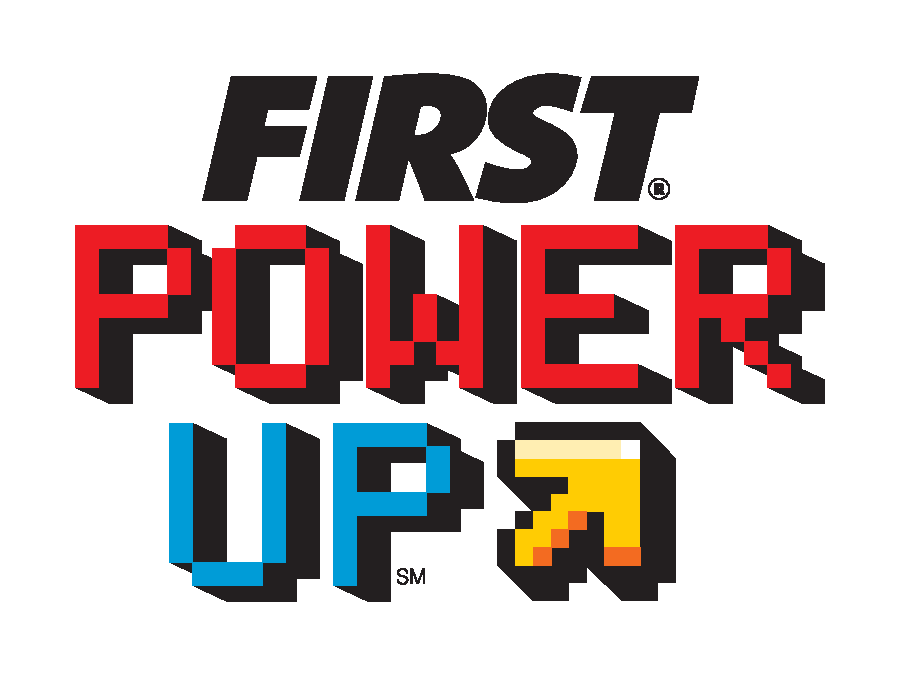
\includegraphics[scale=0.4]{assets/FIRST-FRC18-PowerUp-Stack}
\end{center}

\section{Software Designed for Drivers}
We strive to meld high-performance hardware with custom software to provide our drive team with the best robot possible. Our \textbf{Third Coast Swerve Drive} software has historically provided unmatched manuverability and response but this year's robot design presented the the danger of tipping during intense or sudden teleoperated maneuvers. To counter this danger, the programming team scaled the joystick inputs by applying an exponential scale in addition to the normal deadband.

\begin{figure}[H]
 \centering
 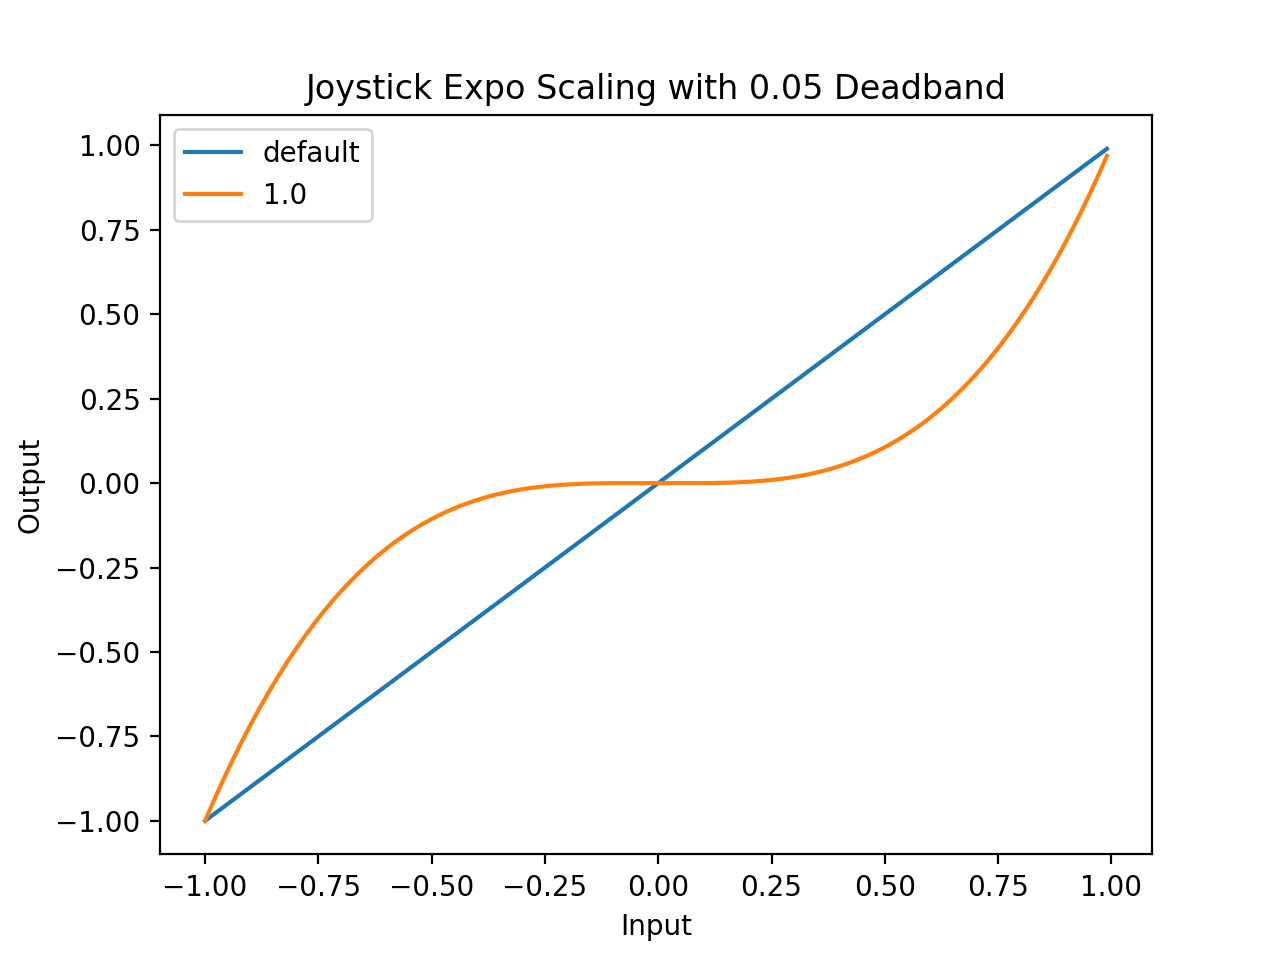
\includegraphics[scale=0.1]{assets/expo}
\end{figure}

Furthermore, the programming team implemented a rate-limiting feature to control the maximum acceleration.  With these features in place, our driver alone would not be able to tip the robot.

\begin{figure}[H]
 \centering
 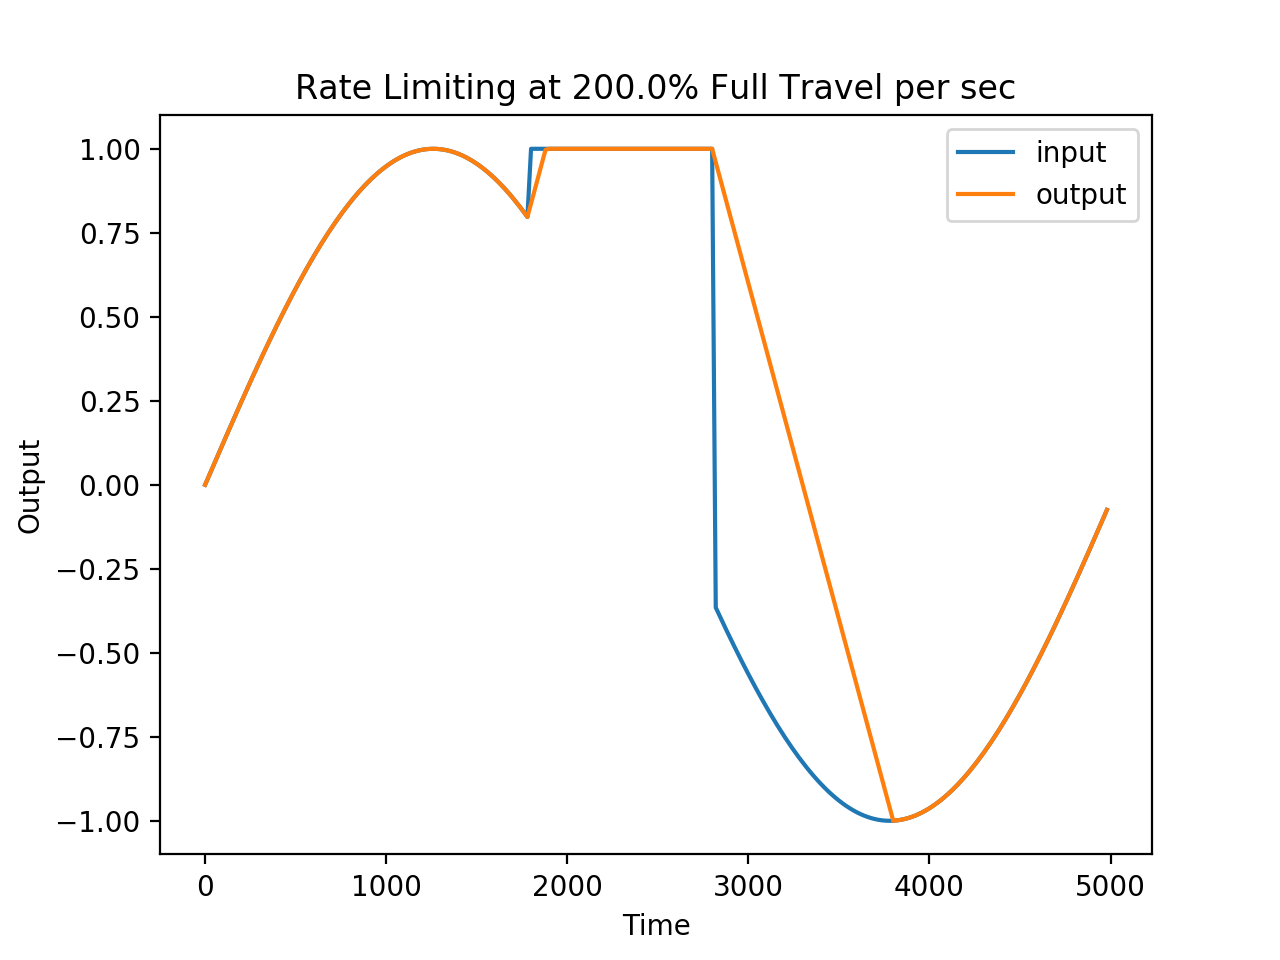
\includegraphics[scale=0.1]{assets/rate}
\end{figure}


\section{Precision Control}

StrykeForce delved deeper into motion profiling this year than ever before.  Using the CTR-Electronics Talon SRX Motion Magic functionality, the programming team controlled the motion-profile by accelerating at a specified acceleration to a setpoint.  This feature in the software allows the robot to make precise and repeatable actuator movements.

\section{``Without Autonomous it's Just a RC Car''}

This (in)famous quote from our senior coach motivates the software team to reach for better autonomous performance every year! This year’s game presented many challenges to the programmers and strategists and required immense cooperation between the two teams.

At first look, the large number of autonomous routines was daunting.  With careful planning, many autonomous paths are built as modules and could easily be reflected and combined for all starting positions and possible field side assignments.  This makes it simple for the programmers to quickly iterate on new autonomous tasks.

\begin{figure}[H]
 \centering
 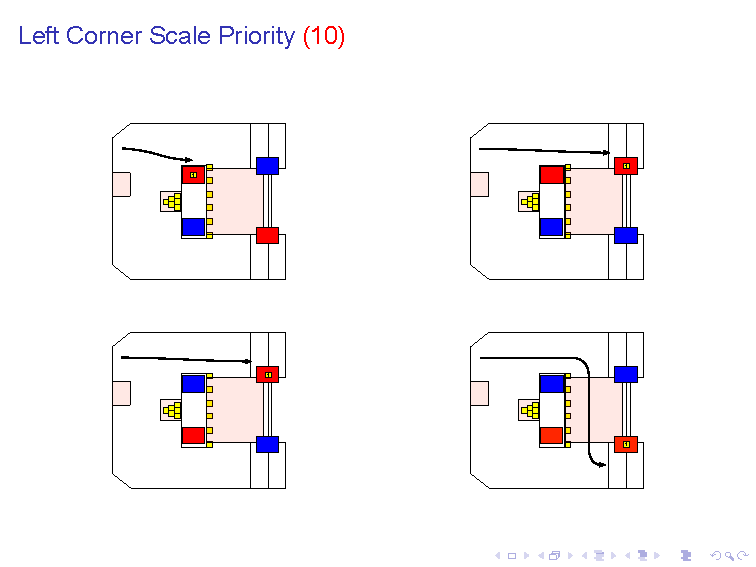
\includegraphics[scale=0.6]{assets/autons}
\end{figure}

To complete the autonomous routines the programming team developed reusable modular commands for movement and controlling actuators that were arranged in command groups to perform more complex parallel tasks and movements.

\section{Autonomous Path Planning}

This year, the programmers used a pathfinding algorithm that fit a cubic hermite spline to a set of waypoints defined by distance in the x and y directions as well as the angle at which to exit to movement.  To make sure the paths worked, the programming team designed and visualized the trajectory waypoints using Python.

\begin{figure}[H]
 \centering
 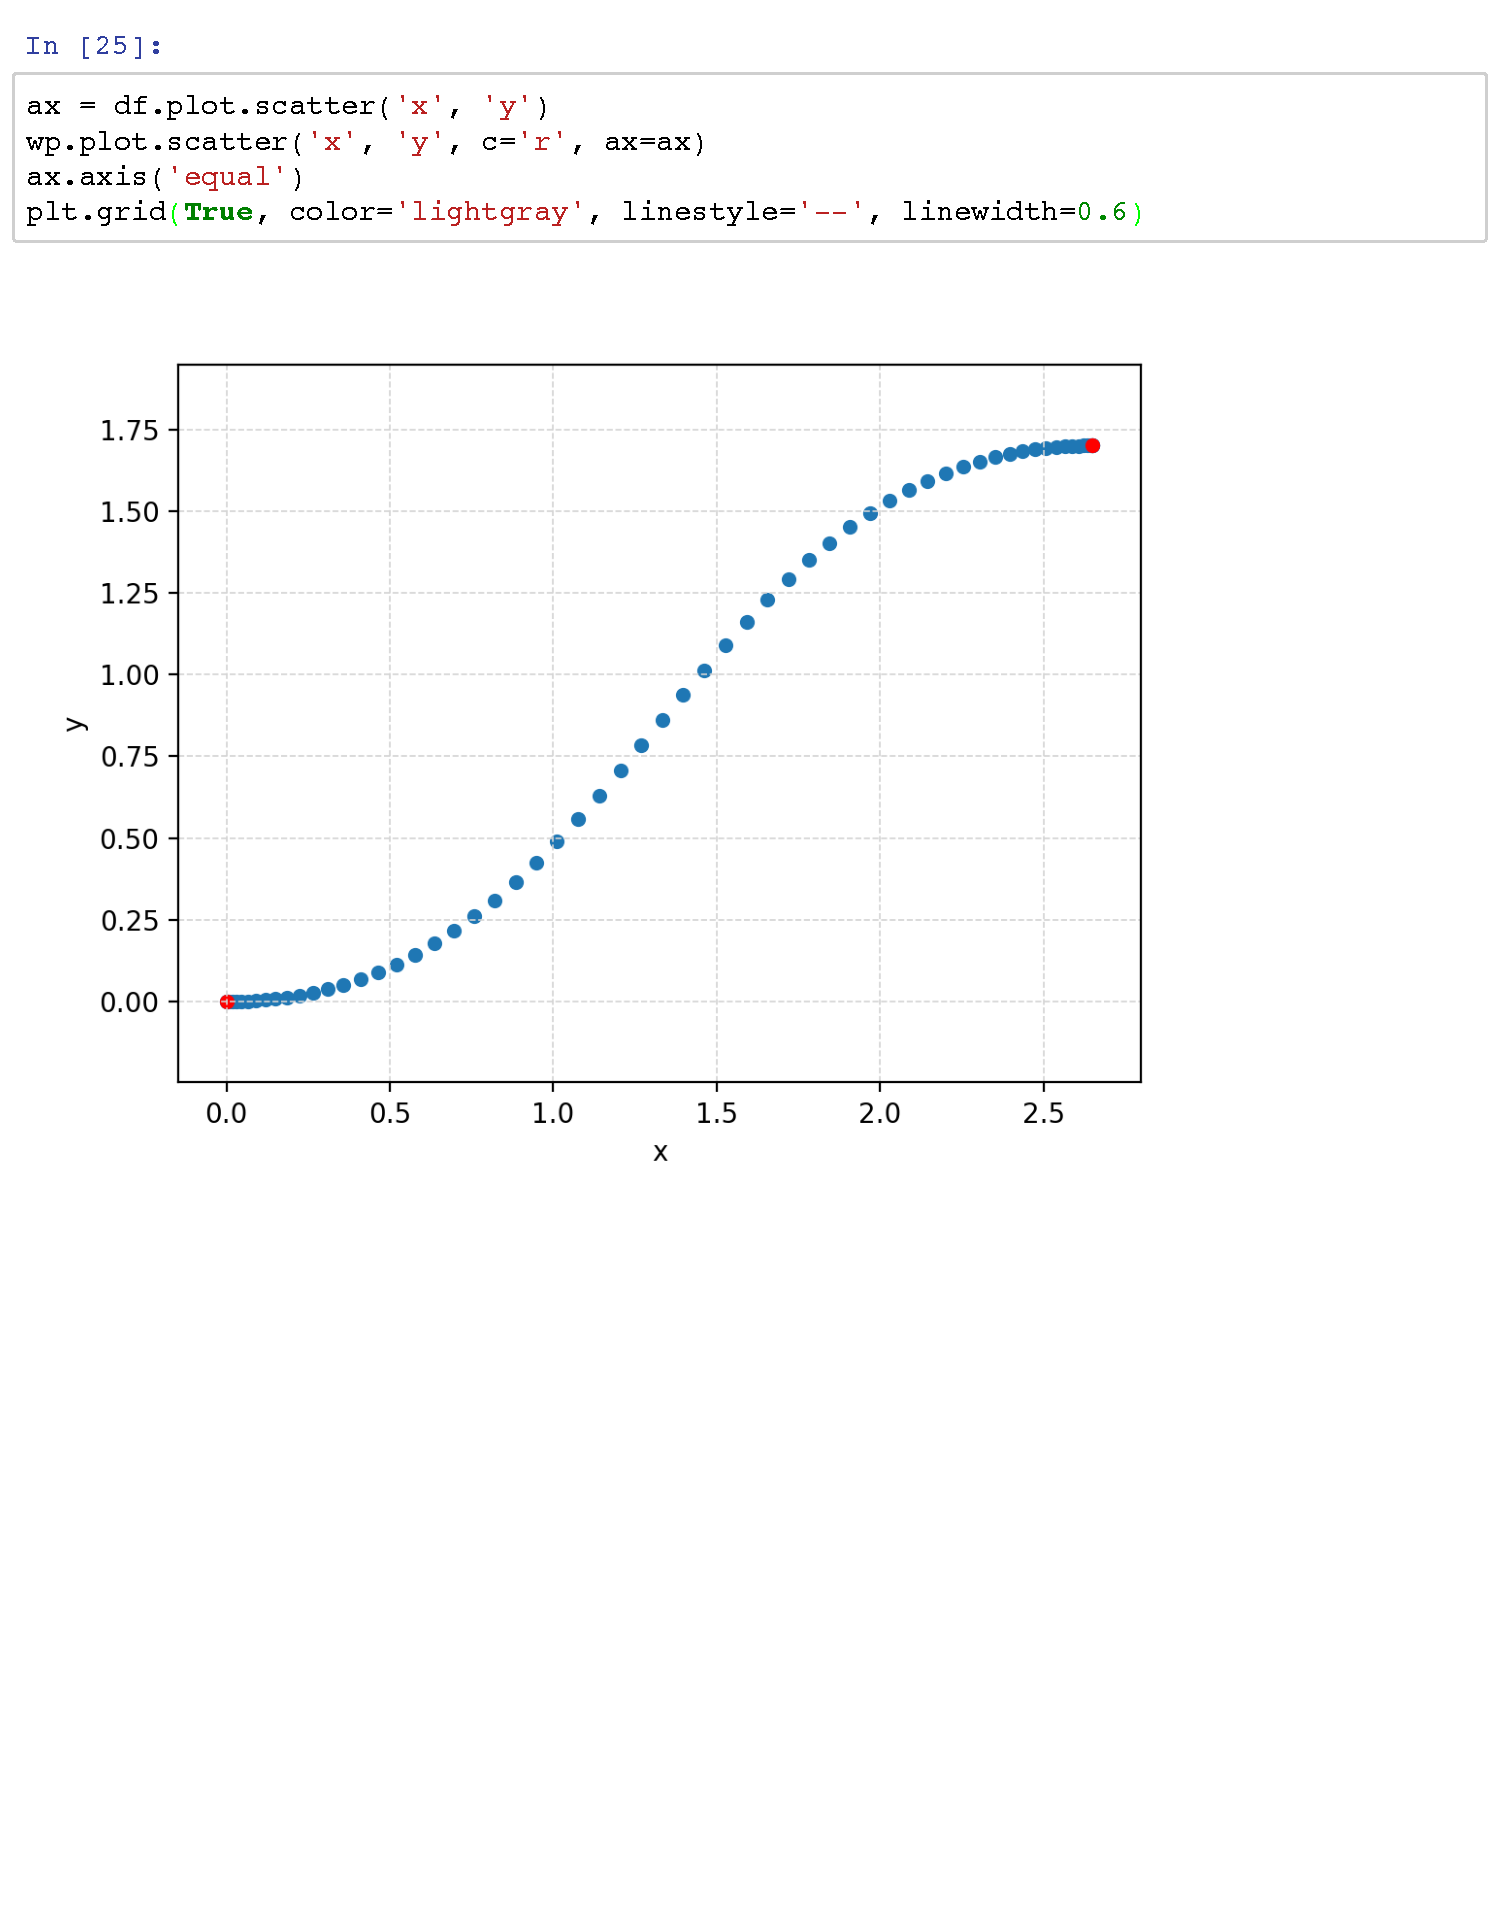
\includegraphics[scale=0.25]{assets/jupyter}
\end{figure}

The path waypoints and motion profiles are managed in a configuration file in the POWER UP project.  When deployed to the RoboRIO, only the paths needed for the specific starting position and desired autonomous routine are calculated during disabled mode to avoid delays once the game begins.

\clearpage

\section{Custom Development Tools}

The software team also builds and maintains custom development tools called \textbf{Third Coast Telemetry} (TCT).  These tools are used by the entire team to test and tune drive systems, actuators and sensors. The Stryke Force Grapher application allows the team to log and analyze the robot performance and perfect the tuning by plotting data received from the roboRIO.  StrykeForce is able to chart almost any data possible from the roboRIO.  TCT and the Grapher applications provide StrykeForce with deep insight into robot performance and are invaluable to the development process.

\begin{figure}[H]
 \centering
 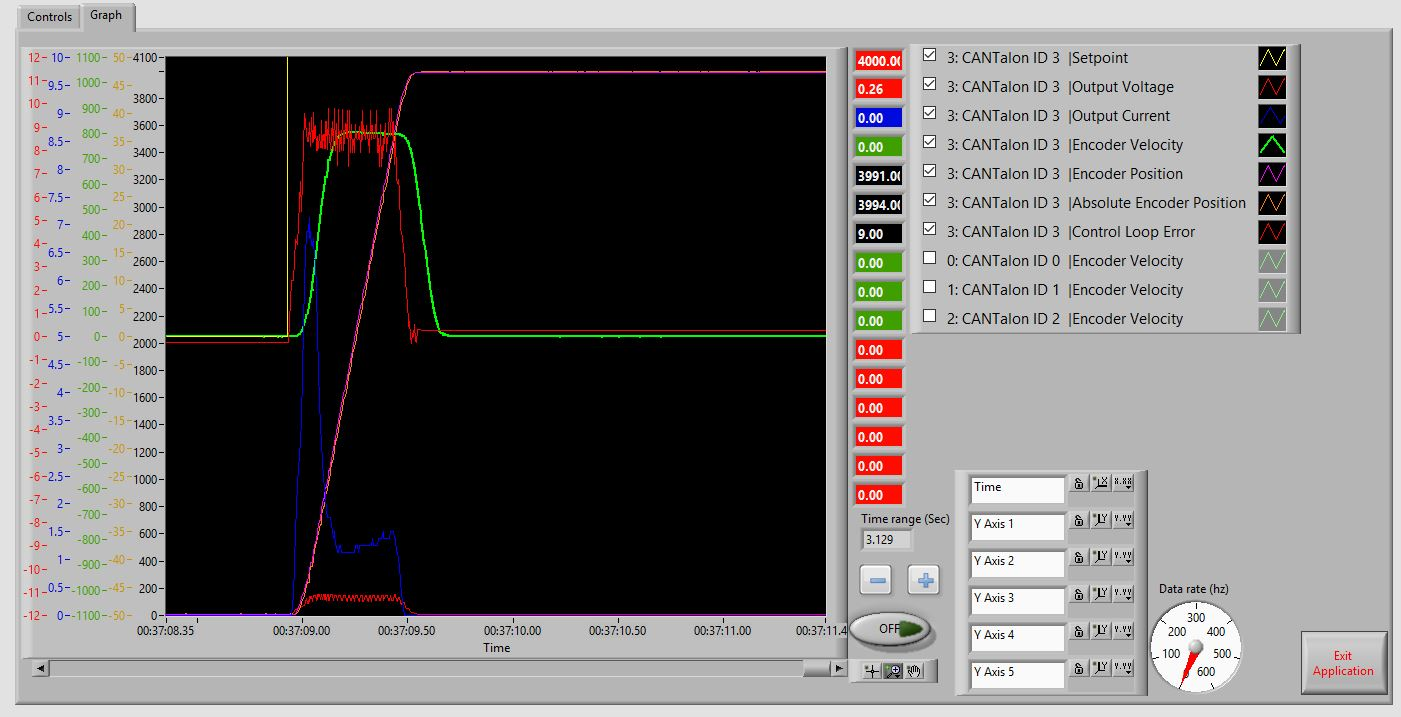
\includegraphics[scale=0.2]{assets/grapher}
\end{figure}

We are pleased to make these tools available as open source at https://github.com/strykeforce.

\section{Software Engineering}

As members of the Stryke Force team, we learn how to work together using real-world tools and processes that will benefit us during our college years and careers ahead.

This year’s FIRST Powerup code is written in Java, an object-oriented programming language and leverages WPILib command-based programming.

The POWER UP project uses GradleRIO, the open-source build automation software.  StrykeForce programmers use Gradle to build projects, deploy code to the RoboRIO, and manage dependencies.

StrykeForce uses GitHub and Git for version control.  The programming team members maintain their own fork of the Powerup and Third Coast repositories.

This year, the programming team adopted the OneFlow Git Branching Model and Workflow.  The programmers maintain one master branch and create pull requests from feature branches they make in their respective forks.  For example, when working on autonomous paths, a programmer would create a new branch in which they would add and modify the autonomous code.  The programmer would then submit a pull request to the master branch in the StrykeForce repository.

\end{document}
